%% example for producing articles in MVA format using LaTeX.
%% written by Takeshi MASUDA, Electrotechnical Laboratory, Japan in May 1996.
%% modified by KAGESAWA Masataka, OKAZAKI Shin'ichro, YASUMOTO Mamoru.
%% last modified by Masaki Onishi, AIST, in Nov 2012.
%% use at your own risk.

\documentclass{mva_style}
\usepackage{graphicx}


\finalcopy %Uncomment this line for the Camera-Ready Manuscript

\begin{document}
\title{Brush Style Transfer with Feedforward Neural Networks}

\author{
  Saki Kohata\\
  Waseda University\\
  Tokyo\\
  {\tt cat-73@akane.waseda.jp}\\
  \and
  Edgar Simo-Serra\\
  Waseda University\\
  Tokyo\\
  {\tt ess@waseda.jp}\\
}

\maketitle

\section*{\centering Abstract}
\textit{
  The emergence of machine learning has revolutionized the world of digital 
  art, providing people with the ability to create highly polished images 
  without advanced drawing skills. 
  However, most of the studies that have been conducted to generate pictures 
  using machine learning are not tools that can be used by people who are 
  already working as creators, such as changing images to artistic styles or 
  generating images based on text. In this study, we propose a model that 
  learns brush styles of human paintings and generates new input images that 
  are redrawn using the learned brush styles. This model is expected to 
  significantly streamline the process of picture creation for creators.
  The generated images by the proposed model are not perfect imitations of 
  the brush style of the reference image. This is thought to be caused by 
  the limitation of the model to generate flexible strokes due to minimal 
  stroke parameters.
  % Our model has the potential to significantly streamline the process of picture creation for creators, offering a powerful new tool for artists and designers alike.
}

\section{Introduction}
Humans have always found value in expressing their feelings and thoughts 
through painting. In order to create excellent works of art, it is necessary 
to learn composition, sketching techniques, colors, lighting effects, etc., 
and it takes a long time to master these skills. However, with the 
advancements in machine learning, it is now possible for people without 
painting skills to generate high-quality paintings. 
For example, Midjourney\cite{Midjourney} is a software application that 
allows users to create wonderful paintings by simply entering words, 
sentences, or keywords that describe the image they wish to have painted. 
Midjourney is popular and highly valued by creators due to its user-friendly 
interface and high-quality results. 
However, it is difficult to say that such a tool is useful for creators who 
have already established their own style. For creators, it is important to 
create works by their own hands, whether digital or analog, and a tool like 
Midjourney, which relies on machine learning for the entire picture creation 
process, is likely to leave creators dissatisfied with the shape and color 
of the drawn objects. Therefore, we aim to conduct research that can support 
creators during their work. Our goal is to develop a model that learns the 
brush style of a picture drawn by a creator and adapts the brush style to a 
new image. In this study, we propose a model that takes two input images, 
a content reference image and a style reference image, and generates an image 
in which what was drawn in the content reference image is redrawn with the 
brush style of the style reference image. 
Figure {fig:haru} shows examples of two input images and an output image.
The picture shown in the content reference image was created with a solid 
coloring brush, so the boundary between colors is always clear. The picture 
shown in the style reference image was created using a brush with a texture 
similar to that of an analog picture, so it is possible to make the 
borderline between colors a gradation. The generated image is a 
representation of the one drawn in the content reference image with the 
brush style of the style reference image.
t is expected that creators can greatly streamline the process of creating 
pictures by manually creating images like the content reference image shown 
in Figure\ref{fig:haru} using a simple brush, and then inputting it into the 
model to have it redrawn with the creator's brush style. Since the content 
reference image is created by the creator, the shape and color of the object 
can be controlled by the creator, and any dissatisfaction with the generated 
image can be resolved with some modifications.


\begin{figure}
  \centering
  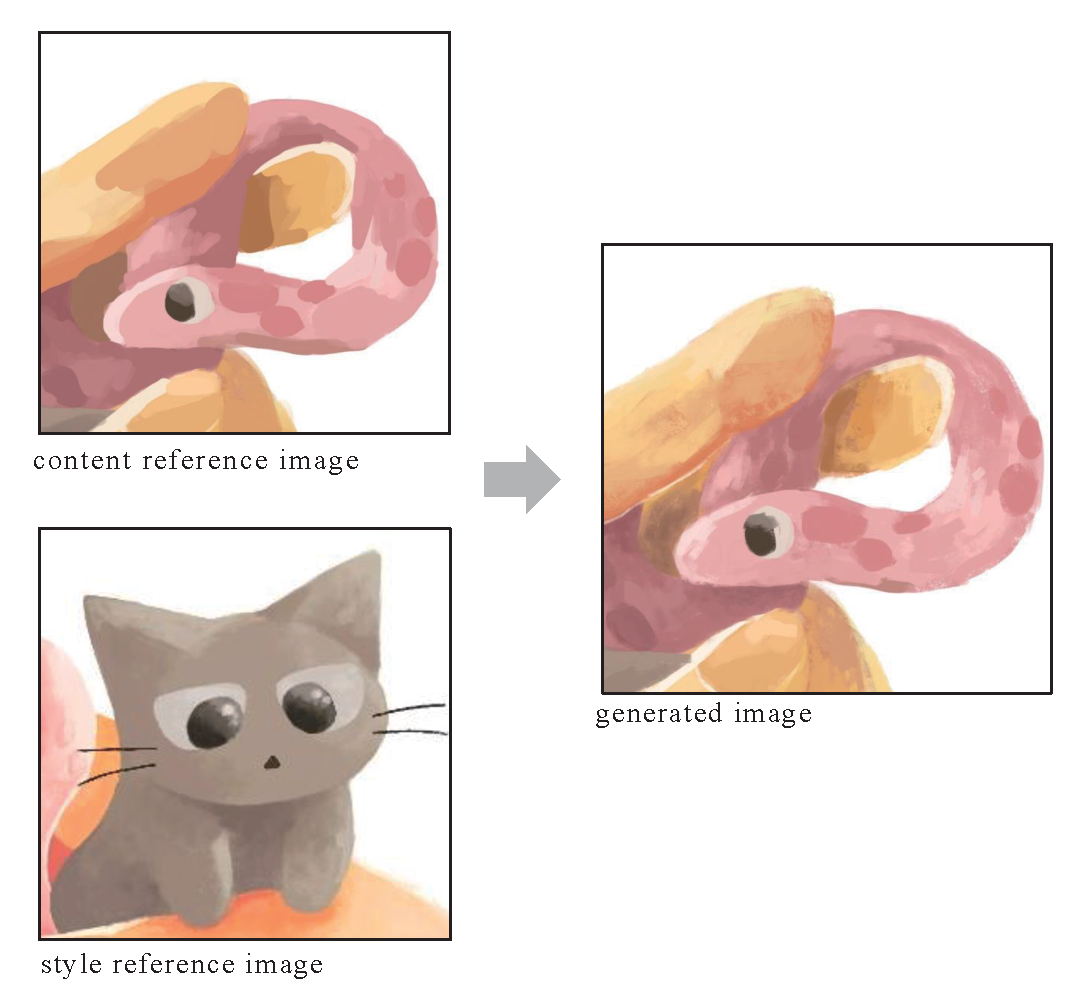
\includegraphics[width=83mm]{resource/haru.eps}
  \caption{Examples of input and output images of the model we would like to create.}
  \label{fig:haru}
\end{figure}

\section{Related Works}
The use of machine learning to generate paintings has been heavily researched 
and has made significant progress. The method using neural networks as a 
generative tool is typically formulated as a pixel-wise mapping \cite{PerceptualLosses} 
or a continuous optimization process in pixel space \cite{ImageStyleTransfer}.
However, it is difficult for neural networks to imitate the way humans both 
create the final image and the process of drawing it. Humans typically start 
by applying rough colors and then gradually adding details, while neural 
networks generate images pixel by pixel. To imitate the human drawing 
process, the machine would have the ability to decompose a given image into 
an ordered sequence of strokes. While neural networks can create sketches 
\cite{DBLP:journals/corr/HaE17}, \cite{DBLP:journals/corr/abs-1805-00247} 
and doodles \cite{DBLP:journals/corr/abs-1810-05977} with a small number of 
strokes, creating a texture-rich painting requires many more strokes.
This makes it difficult to set loss functions for each stroke and prepare 
ground-truth strokes. As a result, Reinforcement Learning (RL) is often used 
to decompose strokes in texture-rich images. \cite{DBLP:journals/corr/abs-1804-01118, DBLP:journals/corr/abs-1206-4634, Huang_2019_ICCV}
Because the computational cost is high in the learning process of an RL agent, 
there are also studies that have formulated this process as a stroke 
parameter search. \cite{PaintTransformer}
The brush style transfers addressed in this paper are similar to those 
addressed in Neural Style Transfer \cite{ImageStyleTransfer}, in which the 
overall mood of an input style image (such as a painting) is transferred to 
another image, using CNNs. The model proposed in that study can transform a 
landscape photograph into an artistic style, but the atmosphere and colors of 
the style reference image as a whole are transferred to the content reference 
image. Therefore, characteristic objects depicted in the style reference 
image, which are not present in the content reference image, appear in the 
output image from the model. 
In this study, we aim to only transfer the style of the brush without changing 
the contents and colors drawn in the content reference image. We addressed 
this issue by adopting the Transformer-based stroke generation pipeline 
proposed by Liu \textit{et al}.\cite{PaintTransformer} as a stroke prediction 
model for our proposed model.

\section{Methodology}
The proposed model utilizes a Transformer-based framework called Paint 
Transformer proposed by Liu et al.\cite{PaintTransformer} as a stroke prediction 
pipeline. The ultimate aim of this research is to create a model that can 
redraw the content depicted in a content reference image using the brush 
style of a style reference image. To achieve this goal, it is necessary to 
alternate the optimization of stroke parameters and brush parameters.
Here, stroke parameters refer to parameters such as the color and size of 
strokes that are different for each stroke, while brush parameters refer to 
parameters common to all strokes, such as the base brush image.
However, at this stage, we have not yet implemented the double optimization.
In the following sections, we will first describe the structure of the 
target model and then present the proposed model.

\subsection{Structure of the target model}
Paint Transformer, used as a stroke prediction pipeline, is a Transformer-based 
framework. This framework generates a sequence of strokes by predicting 
stroke parameters of multiple strokes using a forward propagating transformer.
Paint Transformer consists of two modules: a stroke predictor and a stroke 
renderer. 
A stroke consists of eight parameters: center coordinates $x$, $y$, height $h$,
width $w$, rotation angle $\theta$, and $r$, $g$, $b$ corresponding to RGB values 
representing colors. Thus, stroke $s$ can be expressed as \{ $x$, $y$, $h$, $w$, $\theta$, $r$, $g$, $b$\}.
The strokes rendered by Paint Transformer are monochromatic strokes that are 
scaled, scaled, and rotated from the base brush image. 
Paint Transfomer generates multiple strokes based on eight randomly generated 
parameters and uses them as a training dataset to train a stroke predictor. 
Since the training dataset is generated randomly and automatically, there is 
no need to prepare a dataset. 

数学の話...(疑似latexを読んで)
% 目標のモデルの構造を図\ref{fig:final_model}に示す. 図の上部はストロークパラメータの最適化, 下部はブラシパラメータの最適化の流れである. スタイル参照画像をPaint transformerに入力し, 出力結果を用いてブラシパラメータの最適化を行うことから始める. 次にコンテンツ参照画像をPaint transformerに入力するが, このときに先ほど最適化したブラシパラメータを用いる. その出力結果を用いてストロークパラメータの最適化を行う. これを交互に行うことを繰り返し, ブラシパラメータとストロークパラメータを最適なものに 近づけていく.

\subsection{Structure of the proposed model}
As mentioned earlier, double optimization has not been implemented at this 
stage. In the proposed model, multiple base brush images are prepared, and 
the final output image is the one with the highest similarity of brush style 
with the style reference image among the results of multiple runs of Paint 
Transformer using those images. 
Paint Transformer is used for the stroke prediction model, and a function to 
evaluate the similarity of the style with the style reference image is added 
to the part after stroke prediction by Paint Transformer using the seven 
types of brush images described below.

\subsection{Brush Images}
The model proposed by Liu et al. used a single brush image to generate strokes. 
We newly created six types of brush images. Figure \ref{fig:brushes} shows 
the seven brush images. (a) is the brush image used by Liu et al. and (b)-(g) 
are the newly created ones. In (a)-(c), brush images are provided for each 
horizontal stroke and each vertical stroke.

\begin{figure}[t]
    \centering
    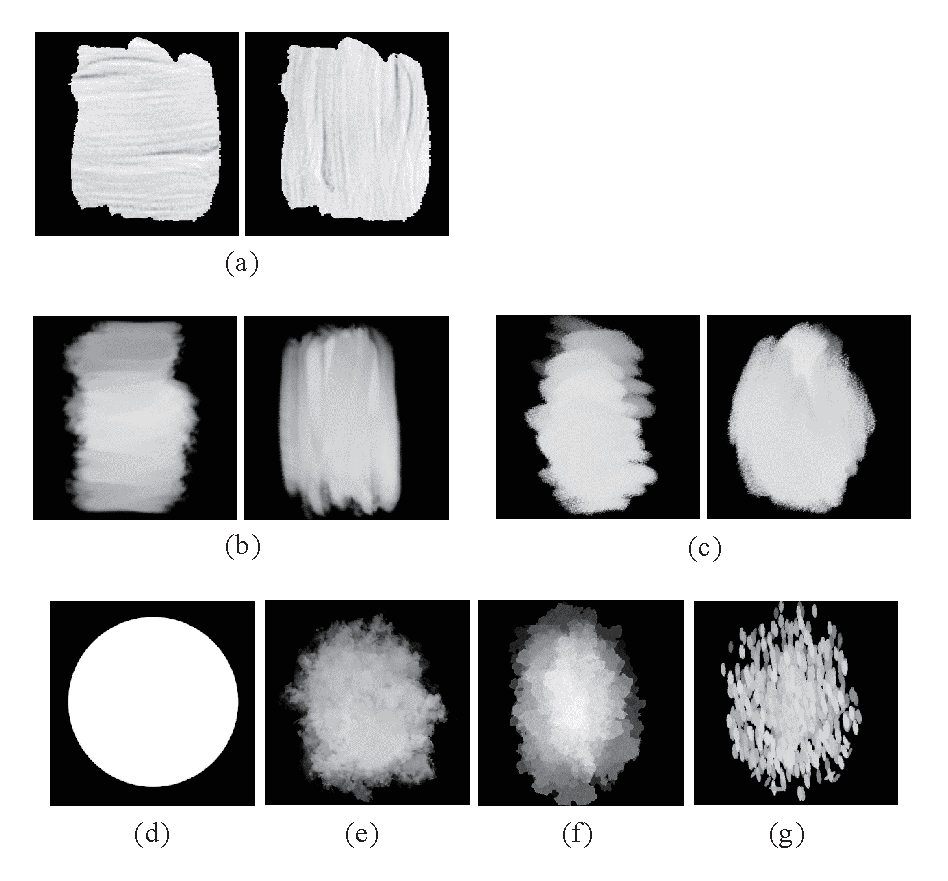
\includegraphics[width=1.0\linewidth]{resource/brushes.eps}
    \caption{Diversity of brushes developed for more accurate representation of painting effects.}
    \label{fig:brushes}
\end{figure}



\subsection{Loss Function}
The $L1$ loss of the Gram matrix is employed as a loss function to evaluate 
the brush style of the output image generated by the Paint Transformer and 
the style reference image. We judged that the Gram matrix is suitable for 
the evaluation of brush styles because it allows us to consider a wide range 
of image correlations.

\section{Experiments and Results}
\subsection{Experiments}
\subsection{Results}
% 結果についてもう少し考察したほうがいいです。またもう少し結果をみせたほうがいいと思います 

\section{Discussions}
\subsection{Future Work}
In this study, we used a Transformer-based framework called Paint Transformer 
to redraw the content drawn on the content reference image using the brush 
style of the style reference image. In the proposed model, since the stroke 
prediction model was trained using Paint Transformer as it is, the stroke 
parameters are the same as those of Paint Transformer, i.e., five shape 
parameters and three color parameters, for a total of eight.In future studies, 
we believe that adding more parameters will enable more flexible brush stroke 
representation. The strokes generated by the proposed model are created by 
scaling and rotating the brush images shown in Figure\ref{fig:brushes}, but 
strokes can also be generated by connecting multiple brush images in 
succession. For example, CLIP STUDIO PAINT \cite{ClipStudio}, a paint software, 
can draw strokes as shown in the lower right of Figure\ref{fig:discussion}, but simply 
adjusting the size of the brush image cannot generate similar strokes, 
resulting in strokes like the one shown in the upper right of Figure\ref{fig:discussion}.
It is expected that by increasing the number of stroke parameters, we can 
increase the expressiveness of the brush and generate strokes like the one 
in the lower right of Figure\ref{fig:discussion}, which imitate the brush style of the 
style reference image. 

\subsection{Conclusion}
In this study, we proposed a novel approach to transform the content of a 
content reference image into a style that imitates the brush style of a style 
reference image using a forward propagating neural network. The final goal 
is to implement a model that iterates optimization of stroke and brush 
parameters in sequence, but the implementation of dual optimization has not 
been achieved. Although the images generated by the proposed model did not 
imitate the brush style of the style reference image, we believe that the 
implementation of the dual optimization will improve the accuracy of brush 
style imitation over the results obtained in this study.
In addition, as described in section 5.1, the small number of stroke parameters 
is also considered to be a point to be improved. Therefore, it is expected 
that the implementation of the dual optimization and improvement in the number 
of parameters will also improve the accuracy of the brush style imitation.

\begin{figure}[t]
  \centering
  
\includegraphics[width=1.0\linewidth]{resource/brush_discussion.eps}
  \caption{Images of the brushes used in the proposed model (left), 
  strokes drawn using Clip Studio Paint (lower right), 
  and a brush image stretched to match the strokes drawn in Clip Studio Paint (upper right).}
  \label{fig:discussion}
\end{figure}


% \begin{table}[t]
%   \caption{Table caption.}
%   \begin{center}
%     \begin{tabular}{c | c c c}
%       \hline
%       \hline
%       \makebox[10mm]{Table} & \makebox[10mm]{1st} & 
%       \makebox[10mm]{2nd} & \makebox[10mm]{3rd}\\
%       \hline
%       1 & 1.0 & 0   & 0 \\
%       2 & 0   & 2.0 & 0 \\
%       3 & 0   & 0   & 3.0 \\
%       \hline
%       \hline
%     \end{tabular}
%     \label{sample-table}
%   \end{center}
% \end{table}

% \begin{figure}[t]
% \noindent
% Long captions should be set as in
%   \begin{center}
%     \includegraphics[height=30mm]{fig2.eps}
%   \end{center}
%   \caption{
%     This is an example of long caption requiring more than one line. 
%     Long captions are placed beneath the figure with a 5 mm 
%     additional margin on both sides.
%   }
%   \label{sample-figure2}
% \end{figure}








\begin{thebibliography}{99}

\bibitem{Midjourney}
“Midjourney,” Accessed: 2023-01-09. [Online]. Available: https://midjourney.com/.

\bibitem{PerceptualLosses}\sloppy
J. Johnson, A. Alahi, and L. Fei-Fei, “Perceptual losses for real-time
style transfer and super-resolution,” \textit{CoRR}, vol. abs/1603.08155, 2016.
arXiv: 1603 . 08155. [Online]. Available: http://arxiv.org/abs/1603.08155.

\bibitem{ImageStyleTransfer}
L. A. Gatys, A. S. Ecker, and M. Bethge, “Image style transfer using
convolutional neural networks,” in \textit{Proceedings of the IEEE Conference
on Computer Vision and Pattern Recognition (CVPR)}, Jun. 2016.

\bibitem{DBLP:journals/corr/HaE17}\sloppy
D. Ha and D. Eck, “A neural representation of sketch drawings,” \textit{CoRR},
vol. abs/1704.03477, 2017. arXiv: 1704 . 03477. [Online]. Available:
http://arxiv.org/abs/1704.03477.

\bibitem{DBLP:journals/corr/abs-1805-00247}
J. Song, K. Pang, Y. Song, T. Xiang, and T. M. Hospedales, “Learning
to sketch with shortcut cycle consistency,” \textit{CoRR}, vol. abs/1805.00247,
2018. arXiv: 1805.00247. [Online]. Available: http://arxiv.org/abs/
1805.00247.

\bibitem{DBLP:journals/corr/abs-1810-05977}
T. Zhou, C. Fang, Z. Wang, J. Yang, B. Kim, Z. Chen, J. Brandt,
and D. Terzopoulos, “Learning to sketch with deep q networks and
demonstrated strokes,” \textit{CoRR}, vol. abs/1810.05977, 2018. arXiv: 1810.
05977. [Online]. Available: http://arxiv.org/abs/1810.05977.

\bibitem{DBLP:journals/corr/abs-1804-01118}
Y. Ganin, T. Kulkarni, I. Babuschkin, S. M. A. Eslami, and O. Vinyals,
“Synthesizing programs for images using reinforced adversarial learn
ing,” \textit{CoRR}, vol. abs/1804.01118, 2018. arXiv: 1804.01118. [Online].
Available: http://arxiv.org/abs/1804.01118.

\bibitem{DBLP:journals/corr/abs-1206-4634}
N. Xie, H. Hachiya, and M. Sugiyama, “Artist agent: A reinforcement
learning approach to automatic stroke generation in oriental ink paint
ing,” \textit{CoRR}, vol. abs/1206.4634, 2012. arXiv: 1206 . 4634. [Online].
Available: http://arxiv.org/abs/1206.4634.

\bibitem{Huang_2019_ICCV}
Z. Huang, W. Heng, and S. Zhou, “Learning to paint with model-based
deep reinforcement learning,” in \textit{Proceedings of the IEEE/CVF Inter
national Conference on Computer Vision (ICCV)}, Oct. 2019.

\bibitem{PaintTransformer}
S. Liu, T. Lin, D. He, F. Li, R. Deng, X. Li, E. Ding, and H. Wang,
“Paint transformer: Feed forward neural painting with stroke predic
tion,” in \textit{Proceedings of the IEEE International Conference on Com
puter Vision}, 2021.


\bibitem{ClipStudio}
“CLIP STUDIO PAINT,” Accessed: 2023-01-09. [Online]. Available: https://www.clipstudio.net/.

\end{thebibliography}



\end{document}
